\chapter{Human-computer interaction}\label{chapter:hci}

\section{Introduction}

When thinking about software design, one often thinks about its rather technical aspects, such as architectures, design patterns and UML diagrams. However, most software will allow interaction between the user and the computer program at least in some way. The types of interaction can range from pressing some buttons on a mircowave to full-fledged graphical user interfaces operated by touching virtual buttons, to giving commands by moving one's eyes to a projected interface, and so on. User interfaces can be very diverse, and so too are the ways one can interact with them. Human-computer interaction is a field on its own within the larger context of computer science and evelops multiple disciplines, including software engineering, psychology, biology and anthropology.

Jakob Nielsen defines human-computer interaction as "a discipline concerned with the design evaluation and implementation of interactive computing systems for human use and with the study of major phenomena surrounding them" [1]. The nature and quality of this interaction relies on several aspects of the machine (or software), as well as the user that operates it. He argues that although good usability is not a guarantee for optimal user satisfaction, in the general case the influence of usability on user satisfaction is large [7].

In the ISO standard \emph{ISO 9241-11}, usability is defined as "the extent to which a product can be used by specified users to achieve specified goals with effectiveness, efficiency and satisfaction in a specified context of use" [10]. Still, usability should not be considered a one-dimensional property of a user interface. Nielsen identifies several characteristics of usability in applications \cite{Nielsen:1993:UE:529793}:
\begin{itemize}
	\item \textbf{Learnability} : if the system is easy to learn, the user can get started quickly;
	\item \textbf{Efficiency} : if the system is efficient to use, it will be possible to complete more work in less time;
	\item\textbf{Error rate and severity} : if the system should be robust and minimize faults;
	\item \textbf{Memorability} : once the system is learned, acquired skills should not be forgotten easily;
	\item \textbf{Satisfaction} : the system should be pleasant to use.
\end{itemize}

In the next sections we will take a closer look at analysis and design techniques for user interfaces, after which we zoom in on usability evaluation techniques for these interfaces.



\section{User interface design}

\subsection{Storyboarding}

A storyboard is a prototype of the system that is composed out of an array of screen sketches. A storyboard describes a particular task , i.e. "story". Note that a user cannot interact with a storyboard, as opposed to paper prototypes [2].


\subsection{Prototyping}

Creating models from an initial design is usually a good way to get a better idea of what the final product will look like and how it will function in reality. Such models can be constructed from various types of materials. The cheapest method to create prototypes is usually by creating paper versions of the various screens of the user interface; this technique will be presented in greater detail in the next section. Alternatively, digital prototypes can be created, for example after testing an initial paper prototype. Since the arrival of 3D printing technology, companies even design and order complete, pysical prototypes. Of course, much will depend on your budget and the type of application you are developing.

In what follows, we elaborate on paper prototyping, based on Carolyn Snyder's book "Paper Prototyping: The Fast and Easy Way to Define and Refine User Interfaces" \cite{Snyder:2003}.

\subsubsection{Paper prototyping}

Carolyn Snyder defines paper prototyping as "a variation of usability testing where representative users perform realistic tasks by interacting with a paper version of the interface that is manipulated by a person 'playing computer', who doesn't explain how the interface is intended to work" \cite{}. It is a technique for designing, testing, and refining user interfaces \cite{Snyder:2003}, and is closely related to usability testing \cite{}. In the last decade it has become a regularly applied technique in major businesses such as IBM, Digital, Honeywell, and Microsoft among others \cite{Snyder:2003}.

In [7] a number of benefits are associated with paper prototyping:
\begin{itemize}
	\item Potential usability problems can be detected at a very early stage in the design process before any code has been written.
	\item Paper prototyping promotes communication between designers and users.
	\item Paper prototypes can be created and refined relatively easily, allowing for rapid design iterations.
	\item Only minimal resources and materials are required.
\end{itemize}

To make your own paper prototype, you will need a number of materials to create the physical paper prototype. Typical materials are blank paper for drawing prototype pieces, some kind of fixed background upon which other paper prototype elements are placed (for example a white poster board sized approximately like a A3 sheet of paper will do), markers, pens (black and/or colored) for hand-drawing the prototype, and scissors for cutting out screen shots into pieces, making popups and so on \cite{Snyder:2003}. Snyder lists also other materials, but feel free to come up with additional materials that can be used to facilitate the simulation of a real interface. An important remark though, is that the paper prototype is usually bigger than the actual interface, and does not have to look very artistic or realistic, as long as it conveys the main ideas of the design \cite{Snyder:2003}.

The background may depend on the application type. A first consideration is whether or not you include elements of the underlying operating system, for example when multiple applications can run simultanously in your test. For most applications, the application interface itself will do. For web browsers buttons such as \textit{Back}, \textit{Forward}, \textit{Home}, and maybe \textit{Print} or \textit{Search} will usually suffice [1]. For small-screen devices where size constraints are important, you can make a so-called 'blinder', which is a print or drawing of the hardware device with a cutout where the display would be \cite{Snyder:2003}.

Having a fixed background for your prototype has several advantages \cite{Snyder:2003}:
\begin{itemize}
	\item It gives a sense of context to what the test subject sees;
	\item If certain controls appear on every screen, you only have to draw them once;
	\item When many pieces of paper are involved in the prototype, it helps the user to distinguish between parts that are on the screen and those that aren't;
	\item It enables you to evaluate the screen real estate.
\end{itemize}

Next the rest of user interface should be added to the background. Different interface controls or widgets can be modeled, such as buttons, checkboxes, tabbed dialog boxes, text fields and drop-down lists. Most of these can be simulated using removable tape, covering some option, or allowing reuse of some widget for the next user test \cite{Snyder:2003}. Note that representing the state of each radio button, list, selection, and so on, is often important as it allows the user to remember his/her choices when using the prototype \cite{Snyder:2003}.

According to Snyder pretty much anything can simulated, using a little imagination. It is still hard to simulate complex or subtle interaction \cite{Snyder:2003}. A number of examples from \cite{Snyder:2003} are listed here:
\begin{itemize}
	\item \textbf{Tooltips/mouseovers} : Tell the users that some visual elements have a tooltip associated with them, and that they can ask if they wish to know what it says for a particular item;
	\item \textbf{Beeps} : Simply say "beep" whenever the computer would, for example, when the user clicks outside a modal dialog box;
	\item \textbf{Drag and drop} : Ask users to specify what they're dragging and where they're dropping it. The Computer then describes the visual changes that occur during this process;
	\item \textbf{Right mouse menus} : Ask users to say when they are clicking the right mouse button. If they do, display the menu.
\end{itemize}


Note that some interactions such as drag and drop, and right mouse clicks often not come to mind of the test subject when using a paper prototype. Also, some interactions such as scrolling are not always incoprporated in the paper prototype, but tested in a later stage of the interface design \cite{Snyder:2003}.

Sometimes hardware can a particular role in the application. For example reading and/or writing to an external device such as a CD or an mp3 player \cite{Snyder:2003}. Snyder argues that including a keyboard is usually not necessary, as most of this can be simulated using simple handwriting with a pen or pencil. If special keys are concerned, ask the test subject how he/she got where he/she is at \cite{Snyder:2003}.



\section{Evaluation methods}

The evaluation of an application prototype can be performed using one or more different techniques, and based on a range of varying criteria, such as: usability, usefulness, meaning, efficiency, accuracy and so on [2]. Based on the slides by Erik Duval, we look at four different evaluation techniques:
\begin{itemize}
	\item Questionnaire;
	\item Usability engineering;
	\item Expert evaluation;
	\item Usage tracking.
\end{itemize}

Methods may be formative or summative. Formative means that the evaluation occurs simultaneously with user task execution. Summative occurs after the user has performed all the required tasks [2].



\subsection{Questionnaire}

A questionnaire is defined as "a method for the elicitation, and recording, and collecting of information" [4]. \textbf{Table} \ref{table:questionnaires} lists several advantages and disadvantages of the use of questionnaires, based on [4].

\begin{table}[H]
	\begin{center}
		\begin{tabular}{l p{300px}}
			\hline
			Advantages		&		Evaluates the point of view of the user; \\
										&		Measures gained from a questionnaire are to a large extent, independent of the system, users, or tasks to which the questionnaire was applied; \\
										&		Quick and cost effective; \\
			\hline
			Disadvantages	&		Only the user's reaction as the user perceives the situation; \\
										&		Lack of detail, as questionnaires are usually designed to fit a number of different situations; \\
										&		Subjective data must be enhanced with performance, mental effort, and effectiveness data. \\
			\hline
		\end{tabular}
	\end{center}
	\caption{Advantages and disadvantages of the questionnaires.}
	\label{table:questionnaires}
\end{table}


\subsubsection{System usabiliy scale}

A system usability scale (SUS) test is a questionnaire that consists out of ten specific questions. Each question is answered by checking one out of five checkboxes: checkbox one corresponds to strong disagreement with the statement, the fifth checkbox corresponds to strong agreement with the statement. The ten questions are listed in \textbf{table} \ref{table:sus_questions}.

\begin{table}[H]
	\caption{System usability scale questions.}
	\begin{tabular}{ p{20px} | p{410px} }
		\hline
		\texttt{Q1} 	&	I think that I would like to use this system frequently. \\
		\texttt{Q2}		&	I found the system unnecessarily complex. \\
		\texttt{Q3}		&	I thought the system was easy to use. \\
		\texttt{Q4} 	&	I think that I would need the support of a technical person to be able to use this system. \\
		\texttt{Q5}		&	I found the various functions in this system were well integrated. \\
		\texttt{Q6}		&	I thought there was too much inconsistency in this system. \\
		\texttt{Q7} 	&	I would imagine that most people would learn to use this system very quickly.  \\
		\texttt{Q8}		&	I found the system very cumbersome to use. \\
		\texttt{Q9}		& I felt very confident using the system. \\
		\texttt{Q10}	& I needed to learn a lot of things before I could get going with this system. \\
		\hline
	\end{tabular}
	\label{table:sus_questions}
\end{table}


\subsection{Usability engineering}

In [2], two methods are described to perform usability engineering tests:
\begin{itemize}
	\item Usability labs;
	\item Think aloud testing;
\end{itemize}

In order to perform reliable usability tests, the test users have to be representative for the actual user population [2]. Often the number of users can be limited to a certain amount. As the number of detectable problems is likely to be finite, from a certain point on adding more users to the usability test will not produce new or better results. Nielsen argues that as a rule of tumb, five test users is enough to acquire reliable and valuable test results [2, 7]. The graph in figure \ref{figure:diminishing_returns} illustrates this phenomenon.

\begin{figure}[H]
	\begin{center}
		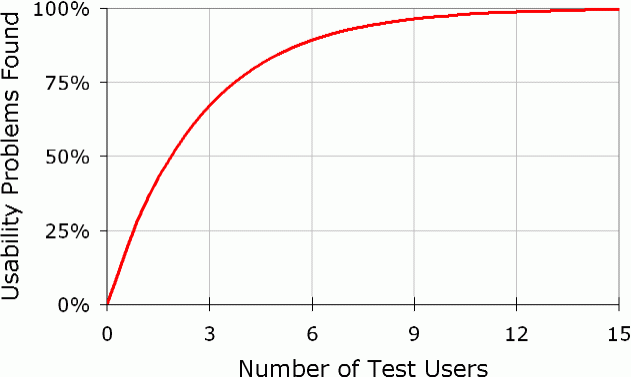
\includegraphics[width=0.6\columnwidth]{img/software-design/user-testing-diminshing-returns-curve}
		\caption{The curve shows the user testing diminishing returns beyond a certain amount of test users.}
		\label{figure:diminishing_returns}
	\end{center}
\end{figure}


The tasks that are being used, have to be representative of the system usage. Tasks also have to correspond to research questions to obtain relevant results.


\subsubsection{Usability lab}

Usability tests can be performed in a usability lab. In this lab the user is observed while performing certain tasks. Data on task completion time, mouse clicks, eye-movement can be collected. Direct observation or cameras can be used to observe the user [3]. To mimic real-life situations, also complete settings can be recreated in which the users would normally use the application.

This method can be rather costly, as labs need to be available and the required equipment may be expensive.


\subsubsection{Think aloud protocol}

A variation on usability lab method that is cheaper to perform, is the think aloud protocol - cf. "discount usability engineering" [2]. To obtain results, the think aloud protocol can be used during a usability test. During a think aloud test, the user describes his/her reasoning for each action he/she undertakes [5]. This method has several advantages and disadvantages, as listed in \textbf{table} \ref{table:usability_engineering}, based on [5] and [9].

\begin{table}[H]
	\begin{center}
		\begin{tabular}{l p{300px}}
			\hline
			Advantages		&		It is cheap to perform; \\
										&		It is robust; \\
										&		It is flexible; \\ % giving required freedom to perform insight tests
										&		It is convincing; \\
										&		It is easy to learn; \\
			\hline
			Disadvantages	&		It creates an unnatural situation, as users usually don't say out loud everything they are about to do or think; \\
										&		The user may tend to filter his/her statements to avoid saying things that he/she may find silly or uninteresting; \\
										&		The facilitator may introduce bias in user behavior if he/she provides too much information when answering or instructing users; \\
			\hline
		\end{tabular}
	\end{center}
	\caption{Advantages and disadvantages of the think aloud protocol.}
	\label{table:usability_engineering}
\end{table}





\subsection{Expert evaluation}

Experts are test users that are spacialists in human-computer interaction or in the application domain itself [2]. Expert analysis is performed by testing the design using guidlines or checklists based on established design principles [2, 10]. In \textbf{table} \ref{table:expert_evaluation} different benefits and drawbacks are listed, based on [2] and [10].

\begin{table}[H]
	\begin{center}
		\begin{tabular}{l p{300px}}
			\hline
			Advantages		&		Quick and relatively cheap feedback that is valid and useful; \\
										&		Promotes compatibility with similar systems; \\
										&		Can be used early in the design process; \\
			\hline
			Disadvantages	&		May be overly critical, as the focus lies on bad characteristics of the design, and as a result, may also be delicate to use with system developers; \\
										&		Restricted to aspects of the interface that are reasonably easy to demonstrate; \\
			\hline
		\end{tabular}
	\end{center}
	\caption{Advantages and disadvantages of the expert analysis method.}
	\label{table:expert_evaluation}
\end{table}



\subsection{Usage tracking}

Systems that have many users can do quick online tests of changes in their software on a subset of its users. By testing on subset of a very large population, much information can be gathered in a small time span.

The main advantages and disadvantages of usage tracking are summarized in table \ref{table:usage_tracking}.

\begin{table}[H]
	\begin{center}
		\begin{tabular}{l p{300px}}
			\hline
			Advantages		&		The context is optimal, as it is the actual environment the user performs the test in; \\
										&		Great quantities of data can be gathered in a short time span; \\
										&		The cost is relatively low; \\
										&		The results are quite accurate; \\
			\hline
			Disadvantages	&		Can only be applied in particular systems; \\
										&		May not provide subjective user feedback; \\
										&		Usually limited to the evaluation of certain interaction types; \\
			\hline
		\end{tabular}
	\end{center}
	\caption{Advantages and disadvantages of usage tracking.}
	\label{table:usage_tracking}
\end{table}





